% THIS IS SIGPROC-SP.TEX - VERSION 3.1
% WORKS WITH V3.2SP OF ACM_PROC_ARTICLE-SP.CLS
% APRIL 2009
%
% It is an example file showing how to use the 'acm_proc_article-sp.cls' V3.2SP
% LaTeX2e document class file for Conference Proceedings submissions.
% ----------------------------------------------------------------------------------------------------------------
% This .tex file (and associated .cls V3.2SP) *DOES NOT* produce:
%       1) The Permission Statement
%       2) The Conference (location) Info information
%       3) The Copyright Line with ACM data
%       4) Page numbering
% ---------------------------------------------------------------------------------------------------------------
% It is an example which *does* use the .bib file (from which the .bbl file
% is produced).
% REMEMBER HOWEVER: After having produced the .bbl file,
% and prior to final submission,
% you need to 'insert'  your .bbl file into your source .tex file so as to provide
% ONE 'self-contained' source file.
%
% Questions regarding SIGS should be sent to
% Adrienne Griscti ---> griscti@acm.org
%
% Questions/suggestions regarding the guidelines, .tex and .cls files, etc. to
% Gerald Murray ---> murray@hq.acm.org
%
% For tracking purposes - this is V3.1SP - APRIL 2009


\documentclass{sig-alternate}

\usepackage[lined,ruled,commentsnumbered,linesnumbered]{algorithm2e}
\usepackage{epstopdf}
\pagenumbering{arabic}
\usepackage{hyperref}
\newtheorem{theorem}{Assumption}

\begin{document}

\title{Distributed File Systems: \\Hadoop Distributed File System and Google File System}
%
% You need the command \numberofauthors to handle the 'placement
% and alignment' of the authors beneath the title.
%
% For aesthetic reasons, we recommend 'three authors at a time'
% i.e. three 'name/affiliation blocks' be placed beneath the title.
%
% NOTE: You are NOT restricted in how many 'rows' of
% "name/affiliations" may appear. We just ask that you restrict
% the number of 'columns' to three.
%
% Because of the available 'opening page real-estate'
% we ask you to refrain from putting more than six authors
% (two rows with three columns) beneath the article title.
% More than six makes the first-page appear very cluttered indeed.
%
% Use the \alignauthor commands to handle the names
% and affiliations for an 'aesthetic maximum' of six authors.
% Add names, affiliations, addresses for
% the seventh etc. author(s) as the argument for the
% \additionalauthors command.
% These 'additional authors' will be output/set for you
% without further effort on your part as the last section in
% the body of your article BEFORE References or any Appendices.

\numberofauthors{2} %  in this sample file, there are a *total*
% of EIGHT authors. SIX appear on the 'first-page' (for formatting
% reasons) and the remaining two appear in the \additionalauthors section.
%
\author{
% You can go ahead and credit any number of authors here,
% e.g. one 'row of three' or two rows (consisting of one row of three
% and a second row of one, two or three).
%
% The command \alignauthor (no curly braces needed) should
% precede each author name, affiliation/snail-mail address and
% e-mail address. Additionally, tag each line of
% affiliation/address with \affaddr, and tag the
% e-mail address with \email.
%
% 1st. author
\alignauthor
Ciprian Lucaci\\
       \email{ciprian.lucaci@tum.de}\\
 	 \affaddr{Technische Universit{\"a}t M{\"u}nchen, Germany}
% 2nd. author
\alignauthor
Daniel Straub\\
       \email{daniel.straub@tum.de}\\
 	 \affaddr{Technische Universit{\"a}t M{\"u}nchen, Germany}
}
% There's nothing stopping you putting the seventh, eighth, etc.
% author on the opening page (as the 'third row') but we ask,
% for aesthetic reasons that you place these 'additional authors'
% in the \additional authors block, viz.

% Just remember to make sure that the TOTAL number of authors
% is the number that will appear on the first page PLUS the
% number that will appear in the \additionalauthors section.

\maketitle
\begin{abstract}
Distributed file systems have been a technology enabler to store and process large files which exceed the size of any drive. They also work in a distributed and fail tolerant manner. The first and most known implementations are Google File System and Hadoop Distributed File System.
\end{abstract}

% A category with the (minimum) three required fields

%A category including the fourth, optional field follows...

\keywords{Distributed File Systems, Distributed Systems} % NOT required for Proceedings

%===========================================
% INTRODUCTION
\section{Introduction}
During the late 90s the Y2K issue was a popular topic in media, but together with the 2000s a bigger and more silent issue took its place. 
The rise of internet traffic, saving and processing every online footprint, having countless of sensors pouring out data into databases and then the rise of the smartphone to a omnipresence status meant that thousands of terabytes and petabytes of data were being generated daily. 
This became a problem due to multiple reasons. Firstly, there was no big enough storage medium to store all the data in a single physical location, and secondly processing such amount of data in order to extract valuable information became an even bigger challenge. Even if there were enough space to store huge amounts of data on a single drive, only seeking through such amount of data would be prohibitive in terms of access times. In this context a new IT domain was born - Big Data. 


The requirements 

Store very large data sets reliably
High bandwidth streaming
Distribute storage
Distribute computation
Analysis and transformation of data

The solution
Moving computation where data resides
Low costs - commodity machines
Vertical and Horizontal scalability

Google File System

Hadoop Distributed File System

\begin{figure}
\centering
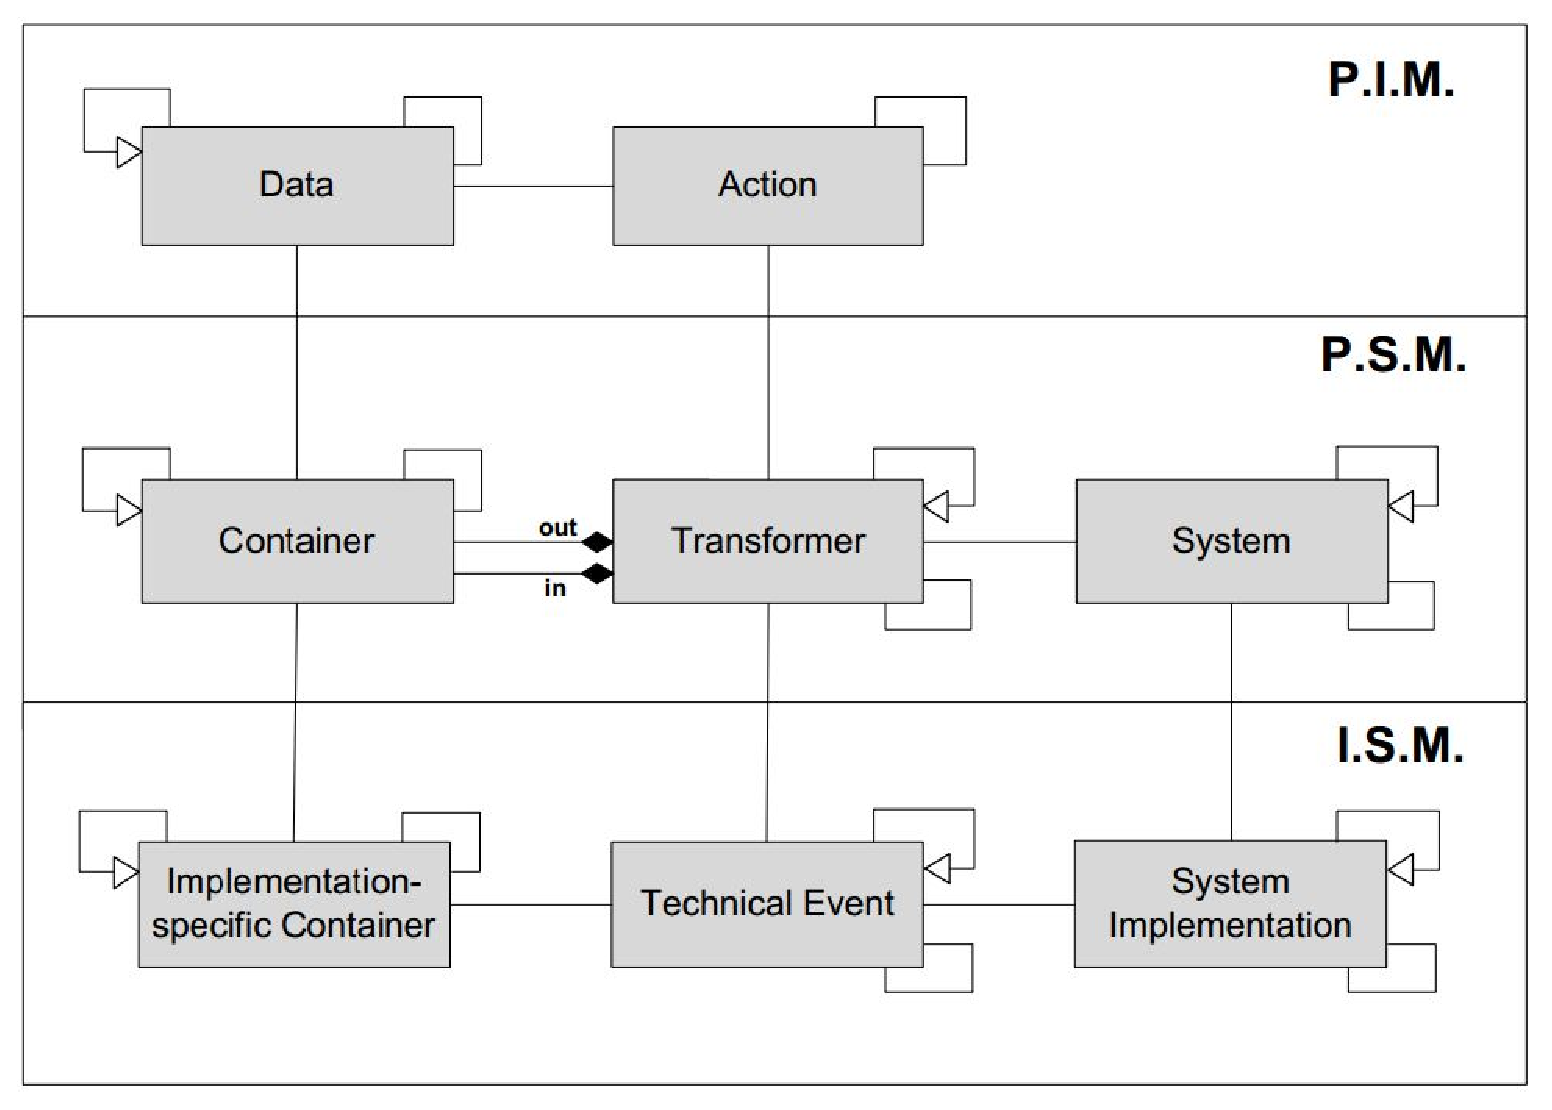
\epsfig{file=domain-meta-model.eps, height=2in, width=3in}
\caption{Domain meta-model}
\label{fig:metamodel}
\end{figure}


%===========================================
% Hadoop
\section{Hadoop Distributed File System (HDFS)}
.. add text cite~\cite{hadoop1}

Hadoop Ecosystem

\subsection{Architecture}
.. add text
\subsubsection{Blocks}
.. add text
\subsubsection{Data Nodes}
.. add text
\subsubsection{Name Node}
master-worker pattern
namespace
Inode
Metadata
Where is the namespace located

\subsubsection{Client}
.. add text
\subsubsection{Secondary Node}
- insert picture
Is there any weakness in the architecture
.. add text
Checkpoint node
Backup node

\subsection{Workflow}
.. add text
\subsubsection{Startup}
\subsubsection{Write}
.. add text code sample
\subsubsection{Read}
.. add text code sample

\subsection{Features}
.. add text
\subsubsection{Block placement policy}
\subsubsection{Replica management}
\subsubsection{Balancer}
\subsubsection{Block scanner}

\subsection{Purpose}
.. add text
Optimized for
- large files
- commodity hardware
- streaming
- batch processing
- multiple reads
Not optimized for
- big amount of small files
- concurrent modification
- arbitrary modification
- general purpose applications
Cross platform
- java, thrift, rest
- web access, console
- opensource
Companies using hdfs
- linkedin, amazon, new york times, twitter, ebay, facebook, spotify, ibm, yahoo


%===========================================
% GFS
\section{Google File System (GFS)}
The Google File System, a distributed file system, was implemented by Google to meet Google's needs. It is widely used within their company.
\subsection{Purpose}
Since the concept of the GFS is the basis of HDFS the purpose of GFS is not much different to the purpose of HDFS. It was designed to store large files, meaning 100 MB and more per file. It should run on commodity hardware, therefore the system has to be fault tolerant. Optimized operations are appending to files and sequential reading of files, which are typical operations when streaming files. The goal of GFS is high data throughput.
While HDFS is open source and widely used by different companies, GFS is not and is only used by Google itself.

\subsection{Architecture}
The GFS consists of three different types of components: the chunkservers, the master and the clients (see figure \ref{fig:gfs_architecture}). While chunkservers store the data which is available in the system, the master controlls the data. The clients can access available data through the master.

\begin{figure}[!hbt]
\centering
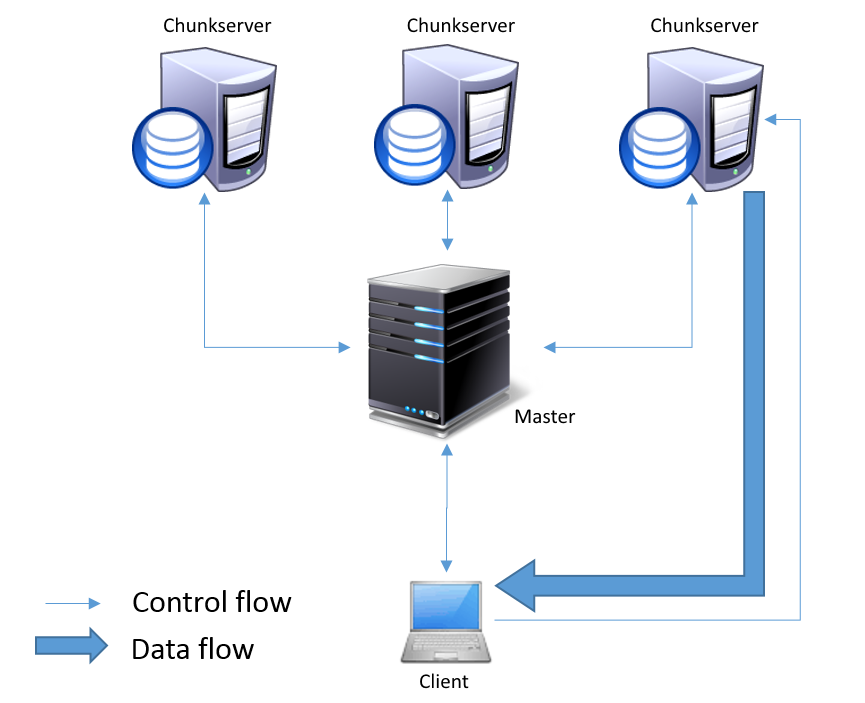
\epsfig{file=gfs_pics/architecture.png, width=\linewidth}
\caption{Google File System Architecture}
\label{fig:gfs_architecture}
\end{figure}

The GFS divides files into chunks of a fixed size. The default chunk size is 64 MB.
Chunks are replicated to increase fault tolerance and load balancing (see \ref{gfs_fault_tolerance_load_balancing}). To identify chunks GFS uses a 64 bit long chunk id which is globally unique.~\cite{google1}

A GFS instance usually consists of many chunkservers which store chunks and one master (see figure \ref{fig:gfs_architecture}). A chunkserver knows about its stored chunks and the corresponding chunk ids. In contrast the master knows about all existing files and which chunks are part of a specific file. Furthermore the master knows where the chunks are stored. It also handles access to chunks as explained in \ref{gfs_workflows}. While the master coordinates access to files, the transmission of data is done directly between a chunkserver and a client. The master is never directly involved in a transmission of data.

\subsection{Workflows}
\label{gfs_workflows}
The GFS allows different operations. The most important ones are \textit{Read}, \textit{Write} and \textit{Record Append}.

\subsubsection{Read}
Reading is the simplest of the mentioned operations and will be explained with figure \ref{fig:gfs_read}.

\begin{figure}[!hbt]
\centering
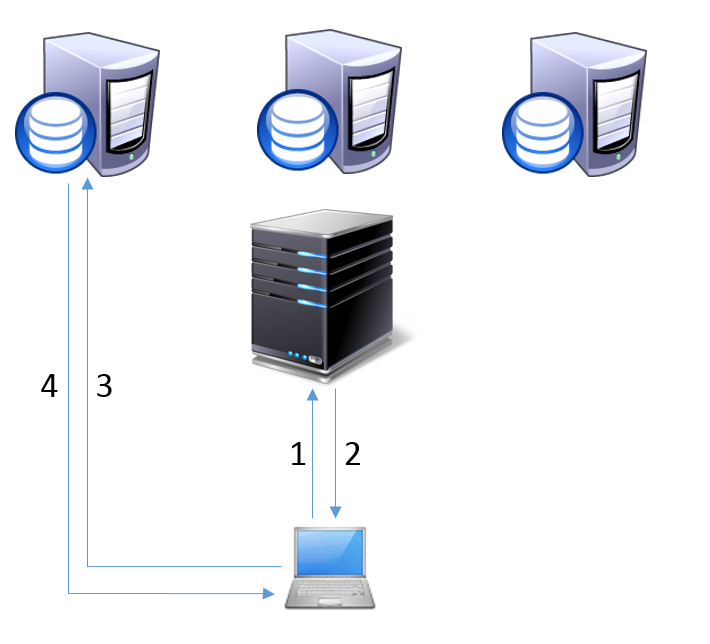
\epsfig{file=gfs_pics/read.png, width=\linewidth}
\caption{GFS read workflow}
\label{fig:gfs_read}
\end{figure}

To read a file, the client first needs to calculate which part respectively chunk it wants to read. This can be done by the client, because the fixed size of the chunks is known system wide. The client calculates for a specific file the chunk index which corresponds to the byte offset it wants to read (not shown in the figure).
Then the client sends a request to the master, containing the name and previously calculated chunk index of the requested file (step 1 in the figure). The master responds with the unique chunk id (see \ref{fig:gfs_architecture}) of the requested chunk and its positions within the system, i.e. the chunkservers containing the requested chunks (step 2). In the 3rd step the client chooses one of the chunkservers and sends a request containing the chunk id and the byte range within that chunk. Finally the chunkserver sends the requested data to the client.

\subsubsection{Write}
\label{gfs_write}
Writing to a file is a bit more complex than the \textit{Read} operation. The \textit{Write} operation can be defined as modifying a specific byte range within a file.

\label{leases}
\textbf{Leases}

GFS uses the mechanism of leases for writing to files. This is done to ensure a consitent mutation order for all replicas of a chunk. A chunkserver may have leases for chunks, but only one chunkserver may have the lease for a specific chunk at any time. The chunkserver which has the lease for a chunk is called \textit{primary}, the others are called \textit{secondaries}. Leases can be requested by chunkservers and are granted by the master.

The following steps explain the execution of a \textit{Write} operation.

\begin{figure}[!hbt]
\centering
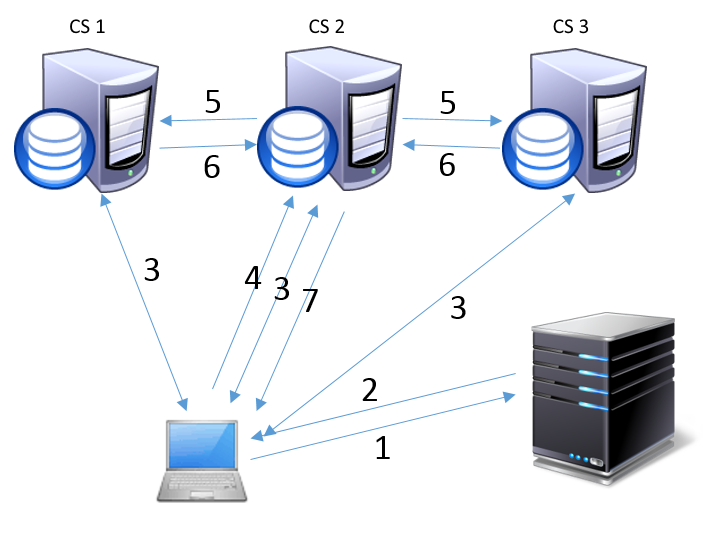
\epsfig{file=gfs_pics/write.png, width=\linewidth}
\caption{GFS write workflow}
\label{fig:gfs_write}
\end{figure}

Assume the following scenario with reference to figure \ref{fig:gfs_write}:

There are three chunkservers (CS), all of them containing the chunk x where x is the unique identifier of the chunk. CS2 is the primary. The master knows that there is a specific file (called file1) which is divided into different chunks with the first chunk being chunk x. It also knows that chunk x is available on the mentioned CSs CS1, CS2 and CS3. The client wants to write to the first byte of file1.

\begin{enumerate}
\item 
Like in the read operation the client's first step is to calculate the chunk index it wants to write to. With the intention to write the first byte of file x the client calculates the chunk index which is 0 (the first chunk of the file). Now the client sends a request to the master containing file name and chunk index (file1, 0).

\item
The master replies with the chunk id, the primary and the secondaries (x, \textbf{CS2}, CS1, CS3). If at this point no CS has the lease for requested chunk, the master grants the lease to one of the chunks before answering the clients request.

\item
With that information the client pushes the data which it wants to write to all replicas (the primary and the secondaries). All receiving CSs write the data to its buffer cache and respond with an acknowledgement for receiving the data.

\item
After all CSs have acknowledged receiving the data, the client sends a write request to the primary. At this point the primary applies the requested write to itself.

\item
Then the primary forwards the write request to all secondaries leading them to apply the changes in the same order.

\item
On successfull writing the data the secondaries will indicate the completion of the write with a response to the primary.

\item
At last the primary returns the result of the write to the client. If there was any error, the client will retry the write from step 3 (pushing the data to CSs). If the error persists, the client will restart from step 1.

\end{enumerate}

\subsubsection{Record Append}
With \textit{Record Append} the GFS provides an atomic write operation. When a client uses this operation to change a file, the client transmits only the data it wants to write, not the position. The CS then decides where the data is written and returns the offset to the client.

The workflow for record append is similar to the write operation explained in \ref{gfs_write}. The differences are in the following steps:

\begin{enumerate}
\item[3.]
The client generally pushes the data to the last chunk of the file.

\item[4.]
Instead of requesting a write, the client sends a record appen request.

\item[5.]
Before the primary applies the changes it checks if the data fits in the chunk (see below). If it fits the following steps are the same as for the write operation.
\end{enumerate}

Something different happens, if the primary's check fails:

If a client wants to append data to a file and the last chunk does not provide enough free space the primary does not apply the changes.

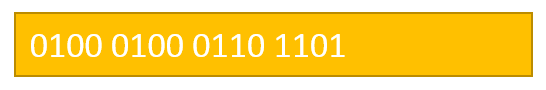
\includegraphics[width=\linewidth]{gfs_pics/writeappend_1.png}

Instead the chunk is padded (e.g. filled up with zeros) and a new chunk is created for the file. The primary then responds to the client with an error asking it to retry the request with the new created chunk.

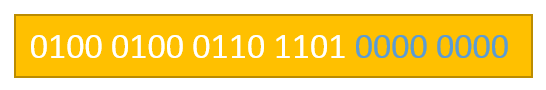
\includegraphics[width=\linewidth]{gfs_pics/writeappend_2.png}

The client will retry, now pushing the data to the new chunk and will succeed.

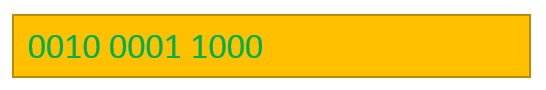
\includegraphics[width=\linewidth]{gfs_pics/writeappend_3.png}

Since the chunk size is limited the record append is technically limited to data with a size of 64 MB or less. GFS further restricts the record append operation to data with no more than one forth of the chunk size. This decision was made to reduce the fragmentation which is created by unsuccessful record append operations.

\subsection{Features}
GFS has a few features implemented to enhance performance and fault tolerance. Chunk replication and garbage collection are two of them which will be explained in the following sections.

\subsubsection{Chunk Replication}
\label{gfs_fault_tolerance_load_balancing}
As mentioned earlier, chunks in the GFS are replicated. By default there are three replicas of each chunk.

\textbf{Chunk Creation:}
When a new chunk is created the master decides where the replicas are placed. This decision is affected by three factors. First new replicas are preferably placed on chunkservers with the most free space. This is done to fill up newly added chunkservers and to have a balanced usage of disk space. Secondly the number creations per chunkserver at any time should not be too high. This avoids flooding new chunkservers with requests. And third the replicas for each chunk should not be on the same rack of chunkservers. This enhances the fault tolerance of the system when whole racks go down e.g. due to network problems.

\textbf{Chunk Re-replication:}
As soon as the number of replicas for a chunk is lower than specified the master will re-replicate it. When re-replicating a chunk the same factors are considered as during the chunk creation. Additionally the re-replication of chunks is prioritized: chunks which have lost more replicas are prioritized to others. Deleted files (see \ref{gfs_gc}) get a lower priority. And at last files currently in use get a higher priority. 

\textbf{Chunk Rebalancing:}
The master periodically checks the distribution of replicas. Depending on chunkserver load and disk space usage the master moves replicas between chunkservers to improve the load and disk space usage.

\subsubsection{Garbage Collection}
\label{gfs_gc}
When a file is deleted in the GFS the master logs the deletion and renames the file, creating a "hidden" file. The deletion time stamp is included in the file name. The garbage collection runs periodically and searches fo files which have been deleted at least three days (default value) ago. Finding such a file results in the final deletion of the file. (figure \ref{fig:gfs_gc})

Until the deletion by the garbage collection the file can still be accessed (using the new file name) or undeleted.

\begin{figure}[!hbt]
\centering
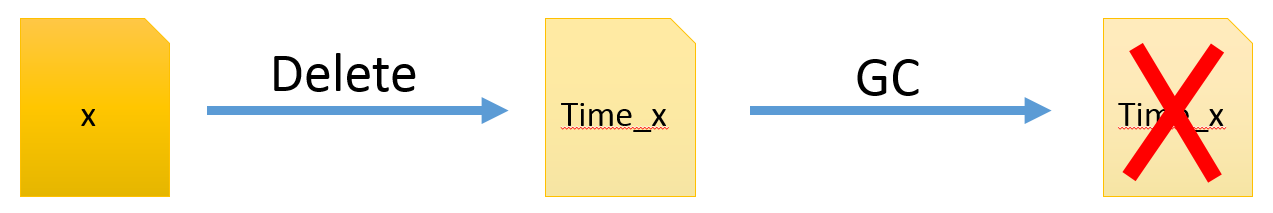
\epsfig{file=gfs_pics/garbagecollection.png, width=\linewidth}
\caption{GFS garbage collection}
\label{fig:gfs_gc}
\end{figure}

%===========================================
\section{Comparison}
Comparing the two distributed file systems, only a closer look uncovers a few differences between HDFS and GFS. But before pointing out these differences a short summary of similarities will be given.\cite{comparison1}

\textbf{Similarities}

Both systems are optimized for operations of the same kind. Processing large files with high performance is one important key feature in the systems. Optimization was done with the assumption that files are written once and read many times. Appending to files has a high performance and guarantees consistency. In contrast modifying files is supported but not seen as important operation and therefore not optimized.
Having these things in mind one can see that GFS and HDFS allow performant streaming of files.

\textbf{Differences}
There are only a few minor differences. GFS allows concurrent appending of files since appending is an atomic operation. This is not the case in HDFS.
The HDFS's namenode is a single point of failure and provides no automatic recovery. In GFS there is the master, which is in some way also a single point of failure. But on a failure the master tries to recover. If this is not working there are also so called shadow masters which can take over operation.
HDFS provides the feature of permission allowing to restrict access to files for different users. The GFS seems not to implement these at the current state.

It can be seen that there are not many differences. The main difference between both systems is the availability: GFS is a proprietary system in contrast to HDFS which is open source.

%===========================================
% CONCLUSIONS
\section{Conclusions and Future Work}
... not finished ...

This paragraph will end the body of this sample document.
Remember that you might still have Acknowledgments or
Appendices; brief samples of these
follow.


%\end{document}  % This is where a 'short' article might terminate


%
% The following two commands are all you need in the
% initial runs of your .tex file to
% produce the bibliography for the citations in your paper.
%===========================================
%BIBLIOGRAPHY
\bibliographystyle{abbrv}

\begin{thebibliography}{4}

\bibitem{hadoop1} Shvachko, K. and Hairong Kuang and Radia, S. and Chansler, R.: The Hadoop Distributed File System, in
\textit{Mass Storage Systems and Technologies (MSST), 2010 IEEE 26th Symposium}, pp.1-10

\bibitem{hadoop2} Hadoop: What it is and why it matters, online at
\url{http://www.sas.com/en_us/insights/big-data/hadoop.html}, [accessed: May 2015]

\bibitem{hadoop3} Hadoop tutorial, online at
\url{http://www.bigdataplanet.info/2013/10/hadoop-tutorials-part-1-what-is-hadoop.html}, [accessed: May 2015]

\bibitem{hadoop4} Thomas Kiencke: Hadoop Distributed File System,
\textit{Institute of Telematics, University of Lubeck, Germany},
 online at
\url{https://media.itm.uni-luebeck.de/teaching/ws2012/sem-sse/thomas-kiencke-hdfs-ausarbeitung.pdf}, [accessed: May 2015]

\bibitem{comparison1} R.Vijayakumari, R.Kirankumar, K.Gangadhara Rao: Comparative analysis of Google File System and Hadoop Distributed File System, in \textit{International Journal of Advanced Trends in Computer Science and Engineering}, Vol.3 , No.1, pp.: 553-558, 2014

\bibitem{google1} Sanjay Ghemawat, Howard Gobioff, and Shun-Tak Leung: The Google File System, in
\textit{Proceedings of the Nineteenth ACM Symposium on Operating Systems Principles, 2003}, pp.29-43

\end{thebibliography}  

%\balancecolumns

\balancecolumns
% That's all folks!
\end{document}
